\chapter[Introdução]{Introdução}
  
  O \textit{MyPush} é uma solução multiplataforma de mensagens instantâneas para troca de informação entre organizações
  e seus usuários finais \cite{cedro15}. O \textit{MyPush} permite ao usuário programar suas notificações sobre apenas o que
  ele deseja de uma organização e pra quando ele deseja. Dessa forma, a plataforma permite que o usuário não receba uma chuva
  de notificações indesejadas, podendo agendar suas notificações sobre seus temas mais utilizados, com um alto nível de
  personalização.
  
  Este trabalho apresenta uma proposta de \textit{design} para o aplicativo \textit{MyPush} para notificações sobre eventos, 
  onde o usuário pode agendar notificações sobre eventos por determinados temas.
  
  \pagebreak
  \section{Cronograma de atividades}
    
    \begin{figure}[!htbp]
      \centering
      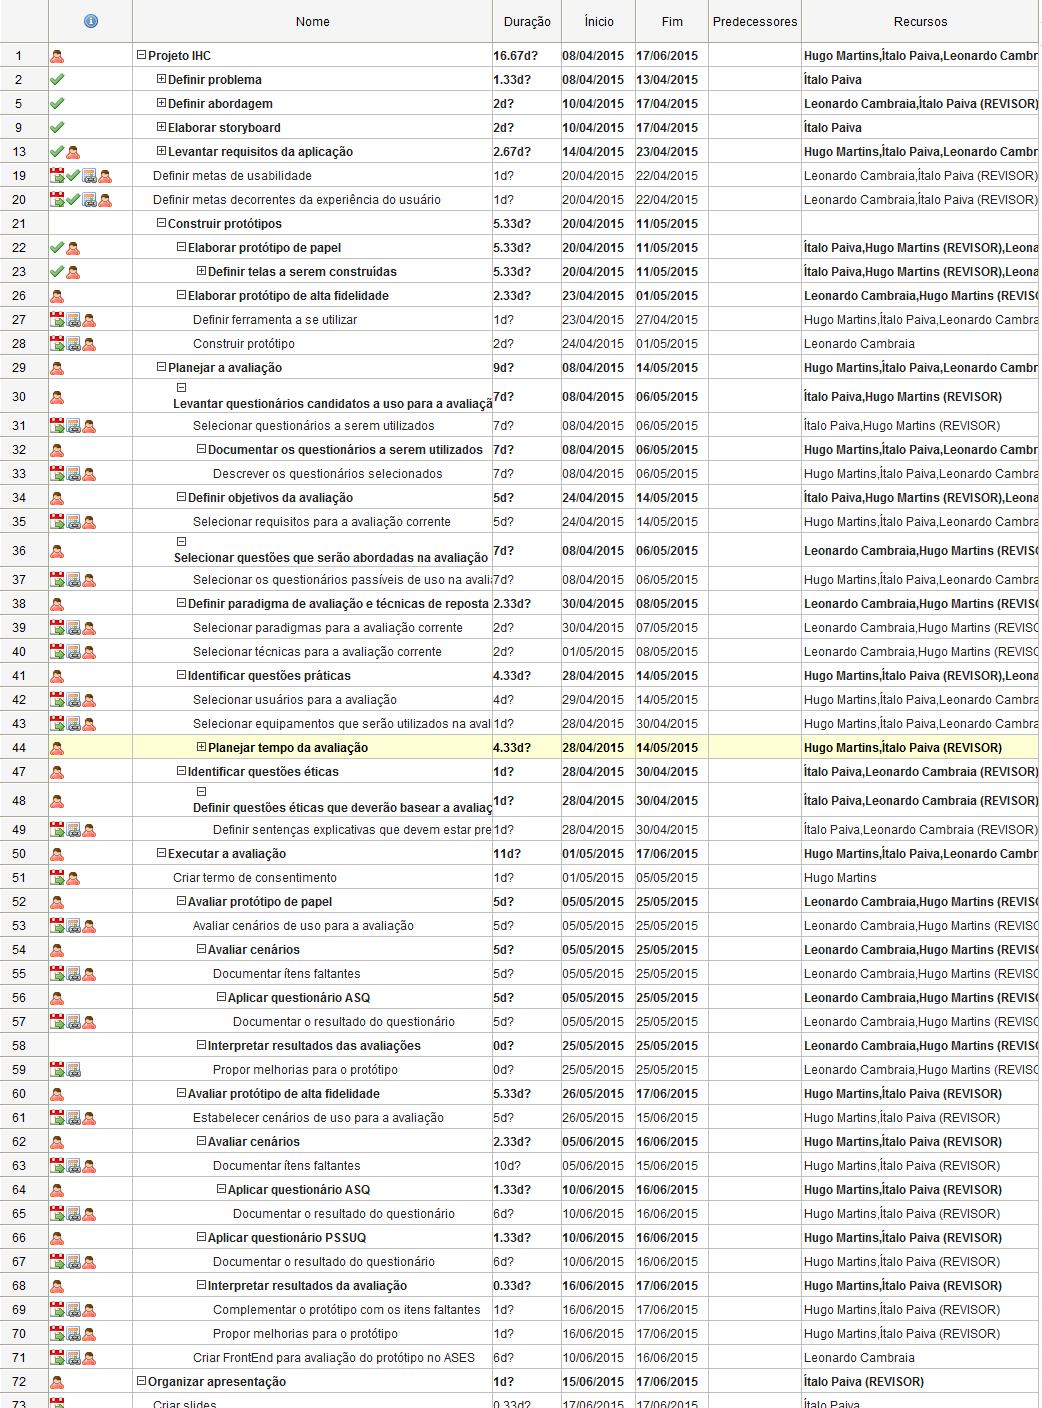
\includegraphics[scale=0.3]{editaveis/figuras/cronograma}
      \caption{Cronograma de atividades}
      \label{cronograma}
    \end{figure}




